%% Factsheet for the MaCVi@WACV 2027 EURS Challenge
%% (Embedded Underwater Restoration and Segmentation)
%%
%% Team: SAT (Institution: MIT-BLR / Manipal Institute of Technology Bengaluru)
%% Best Models: Track 1 (V33-Ensemble-F3Upgrade, Sub #19359 | 0.641)
%%              Track 2 (track2-apex-orin-v3, Sub #19447 | 0.407)

\documentclass{article}

\usepackage[margin=2.5cm]{geometry}
\usepackage{graphicx}
\usepackage{colortbl, color, xcolor}
\usepackage{hyperref}
\usepackage{amsmath}
\usepackage{booktabs}
\usepackage{tabularx}
\usepackage{enumitem}
\usepackage{ifthen}

% ---- switches -------------------------------------------------------------
\newboolean{showinstructions}
\setboolean{showinstructions}{false}   % set to false for the PDF you send

% Red placeholder text: no remaining placeholders in final submission
\newcommand{\todo}[1]{\textcolor{red}{[#1]}}

\date{October 28, 2026}
\title{\textbf{MaCVi@WACV 2027 EURS Challenge\\Embedded Underwater Restoration and Segmentation\\Factsheet}}

\author{Arin Pattnaik, Tanmay Das, Shubham Kulkarni, Dr. Chaitra Desai\\
\small Department of Computer Science \& Engineering, Manipal Institute of Technology (MIT-BLR),\\
\small Manipal Academy of Higher Education, Bengaluru, Karnataka, India}

\begin{document}

\maketitle

% =============================================================================
% INSTRUCTIONS (hidden when showinstructions=false)
% =============================================================================
\ifthenelse{\boolean{showinstructions}}{%
\section*{Instructions: how to submit the factsheet}
[Instructions hidden]
\newpage
}{}

% =============================================================================
\section{Team details}\label{sec:team}
\begin{itemize}[leftmargin=*]
\item \textbf{Team name (as on macvi.org):} SAT (MIT-BLR)
\item \textbf{Team leader name:} Arin Pattnaik (Faculty Advisor / Mentor: Dr. Chaitra Desai)
\item \textbf{Team leader institution and email:} \\
Department of Computer Science \& Engineering, Manipal Institute of Technology (MIT-BLR), Manipal Academy of Higher Education, Bengaluru, Karnataka, India \\
Email: \texttt{arinp2018@gmail.com} (Faculty Email: \texttt{chaitra.desai@manipal.edu})
\item \textbf{Rest of the team members (name, macvi.org user ID):}
  \begin{itemize}
    \item Arin Pattnaik (Team Owner on macvi.org), user ID \texttt{2044}
    \item Tanmay Das, user ID \texttt{2043}
    \item Shubham Kulkarni, user ID \texttt{2035}
    \item Dr. Chaitra Desai (Faculty Advisor \& Mentor)
  \end{itemize}
\item \textbf{Team website URL (if any):} \url{https://github.com/syntax-error23/SAT-EURS}
\item \textbf{Affiliations:} Department of Computer Science \& Engineering, Manipal Institute of Technology Bengaluru (MIT-BLR), Manipal Academy of Higher Education, Bengaluru, Karnataka, India
\item \textbf{Team leader's user ID on the submission server (macvi.org):} \texttt{2044}
\item \textbf{User IDs on the submission server of all team members (leader included; the IDs of every account that submitted for the team):} \texttt{2044}, \texttt{2035}, \texttt{2043}
\item \textbf{Track(s) entered:} both (Track 1 and Track 2)
\item \textbf{Best-scoring testing-phase submission per track (the one reported for reproduction):}
  \begin{itemize}
    \item Track 1 (testing-phase submission used for the final ranking): submission ID \textbf{\#19359}, submitted by user ID \texttt{2035} (\texttt{shubham.kulkarni232007@gmail.com}), composite score \textbf{0.6410} ($Q_{\text{seg}}$: 0.5820, mIoU: 0.7110, Macro $F_1$: 0.8180, PSNR: 25.48 dB, SSIM: 0.8290)
    \item Track 2 (testing-phase submission used for the final ranking; Jetson AGX Orin, ONNX): submission ID \textbf{\#19447}, submitted by user ID \texttt{2044} (\texttt{arinp2018@gmail.com}), composite score \textbf{0.4070} ($Q_{\text{seg}}$: 0.2270, mIoU: 0.4060, Macro $F_1$: 0.5600, PSNR: 23.25 dB, SSIM: 0.8470, Complexity: 9.82 GFLOPs, 0.884 M params)
  \end{itemize}
\item \textbf{Link to the reproduction repository (created from the official EURS template, one per track entered):}
  \begin{itemize}
    \item Track 1 (Unconstrained Quality): \url{https://github.com/syntax-error23/SAT-EURS-Track1-Repro}
    \item Track 2 (Jetson AGX Orin Edge): \url{https://github.com/syntax-error23/SAT-EURS-Track2-Repro}
  \end{itemize}
\item \textbf{Artifact traceability:}
  \begin{itemize}
    \item Code revision / commit: \texttt{9633b4d}
    \item Track 1 final submission archive: \texttt{deploy/v33/submission\_v33\_ensemble\_f3upgrade.zip} \\
    SHA-256: \texttt{de741a84ce4601f82286ef156458b07e9fe2d4c4f75559a4589010f90ae6510d} (498.01 MB, 1,200 JPEGs + 1,200 PNG masks)
    \item Track 2 submitted ONNX binary: \texttt{deploy/track2\_apex\_orin\_v3.onnx} \\
    SHA-256: \texttt{addf76f170a0c09e0a3af50ebabb530b3f542080d2f3921c171ea3ae3cd80247} (6.79 MB static graph)
    \item Link access status: Public GitHub repository, permanent access.
  \end{itemize}
\end{itemize}

% =============================================================================
\section{Global method description}\label{sec:global}

Optical degradation in underwater imaging is governed by wavelength-dependent absorption and severe forward/backward scattering. Coupling physical radiative transfer inversion directly with deep categorical segmentation often causes severe gradient competition: restoration rewards pixel-level high-frequency reconstruction, whereas dense segmentation requires semantic spatial invariance. To resolve this, our methodologies differ strategically across the two tracks:

\paragraph{Track 1 (Unconstrained Quality):} We deploy a sequential decouple-and-fuse architecture. Restoration is anchored physically via an analytical 19-term polynomial basis ($\phi(r,g,b) \in \mathbb{R}^{19}$) regressed via closed-form Tikhonov regularisation ($\lambda = 10^{-4}$), ensuring baseline color recovery without high-frequency amplification. A neural refiner consisting of 16 Non-Linear Activation Free (NAF) blocks~\cite{chen2022nafnet} with depthwise gated convolutions operates on the concatenated 8-channel tensor [Raw RGB, RSUIGM RGB, Water Type, Depth]. To prevent distribution shift, the refiner output is strictly bounded: $I_{\text{rest}} = \text{clip}(I_{\text{RSUIGM}} + 0.10 \times \tanh(\text{NAFNet}), 0, 1)$, followed by Laplacian unsharp edge filtering ($\alpha=1.34, \sigma=1.5$), reaching 25.48\,dB PSNR and 0.829 SSIM. For segmentation, our \texttt{EURSAPEXV18Segmenter} deploys an asymmetric dual-stream encoder: (1) DINOv3 ViT-Large/16 (304\,M params)~\cite{oquab2023dinov2} ingests restored images at $518\times518$ for global semantics, (2) ConvNeXt-Base (88.5\,M params)~\cite{liu2022convnet} ingests raw degraded images at $512\times512$ with a 2-stage DetailStem to eliminate the typical 10--15 pixel ViT boundary dilation on thin fauna, and (3) learned spatial gating $f_{\text{fused}} = \sigma(G) \odot f_{\text{sem}} + (1 - \sigma(G)) \odot f_{\text{conv}}$ with condition FiLM modulation across a 4-level UPerNet feature pyramid.

\paragraph{Track 2 (Jetson AGX Orin Edge SOTA):} Under the strict $\le 1.0$\,M parameter and $\le 12.0$\,GFLOP limits, separate heavy models are impossible. Track 2 adopts a unified multi-task architecture: (1) an 18-D radiometric summary router computes translation-invariant global statistics from a downsampled $256\times256$ representation and contracts against a scale-consistent 20-scene calibration bank in $<0.30$\,GFLOPs (a 95\% compute saving over 2D convs), (2) a 3-block depthwise-separable inverted bottleneck refiner operating at $256\times256$ with condition FiLM modulation lifts PSNR from 17.1\,dB to 23.25\,dB ($+6.15$\,dB), (3) a shared dual stem feeds a MobileNetV3-Large trunk~\cite{howard2019mobilenetv3} \textbf{truncated strictly after Block 11} (\texttt{features[:12]}), eliminating Block 12's heavy 386\,k parameter expansion and keeping total parameters at 884.1\,k (passing the 1.0\,M ceiling with 11.6\% headroom), (4) a dilated ASPP context module and 4-scale progressive FPN, and (5) an in-graph average pooling speckle suppressor ($\text{AvgPool2d}(11, 1, 5)$) that penalizes rare-class logits where regional support is below $\tau=0.04$, executing natively on TensorRT with 0 extra parameters.

\begin{itemize}[leftmargin=*]
\item \textbf{Which pre-trained or external methods / models have been used:}
  \begin{itemize}
    \item DINOv3 ViT-Large/16 pre-trained on LVD-142M via self-supervised learning~\cite{oquab2023dinov2}.
    \item ConvNeXt-Base pre-trained on ImageNet-1k~\cite{liu2022convnet}.
    \item MobileNetV3-Large pre-trained on ImageNet-1k~\cite{howard2019mobilenetv3}.
    \item NAFNet architecture blocks~\cite{chen2022nafnet}.
  \end{itemize}
\item \textbf{Which additional data has been used in addition to the provided EURS training data:} \textbf{None}. Strictly trained exclusively on the provided EURS benchmark scenes (20 training scenes, 6 dev scenes). No external imagery, synthetic generators, or unannounced data were used.
\item \textbf{Training description:}
  \begin{itemize}
    \item \emph{Framework:} PyTorch 2.11 / 2.6 with CUDA 12.8, torchvision 0.26.0, timm 1.0.30.
    \item \emph{Optimizer:} AdamW ($\beta_1=0.9, \beta_2=0.999$, weight decay $10^{-4}$).
    \item \emph{Learning rate schedule:} Cosine annealing with 3 warmup epochs; peak learning rate $3\times10^{-5}$ for Track 1, $2\times10^{-4}$ for Track 2; minimum learning rate $10^{-6}$.
    \item \emph{Batch size:} Effective batch size 16 for Track 1 (batch size 4 with 4 gradient accumulation steps); batch size 8 for Track 2.
    \item \emph{Epochs:} 25 epochs per fold for Track 1; 30 epochs for Track 2.
    \item \emph{Input size:} $518\times518$ (ViT stream), $512\times512$ (ConvNeXt stream), $1024\times1024$ (Restoration and Track 2 edge model).
    \item \emph{Augmentations:} Random horizontal/vertical flips, scale jittering $[0.8, 1.25]$, random crop, subtle color jitter (brightness, contrast, saturation $\pm0.1$), and targeted copy-paste rare organism oversampling on elasmobranchs.
    \item \emph{Loss functions and weights:}
      \begin{itemize}
        \item Track 1: Present-Class Lov{\'a}sz-Softmax ($w=1.0$)~\cite{berman2018lovasz}, Class-Weighted Focal Cross-Entropy ($\gamma=2.0, \alpha=[0.70, 0.90, 1.20, 3.00, 3.50], w=1.0$)~\cite{lin2017focal}, Soft Dice Loss ($w=0.5$), Auxiliary Boundary BCE ($w=0.2$), and L1 + Laplacian high-frequency restoration loss ($w=0.1$).
        \item Track 2: Multi-Teacher Ensemble Distillation ($L_{\text{KD}}$, temperature $\tau=3.0, w=1.0$), Present-Class Lov{\'a}sz-Softmax ($w=1.0$), Soft Dice ($w=0.5$), and Restoration L1 + Laplacian Loss ($w=0.2$).
      \end{itemize}
    \item \emph{Hardware:} Single NVIDIA GeForce RTX 5090 (32GB VRAM, Blackwell architecture), 64GB DDR5 host memory.
    \item \emph{Training time:} Track 1 $\approx 18$ hours across all 5 cross-validation folds; Track 2 $\approx 3.5$ hours for 30 epochs.
  \end{itemize}
\item \textbf{Testing description:}
  \begin{itemize}
    \item \emph{Resolution:} Full native resolution. Inputs are resized such that the longest side is exactly 1024\,px, aspect ratio preserved, strictly matching the official scoring protocol.
    \item \emph{TTA / Ensembling:} Track 1 uses a 5-fold cross-validation ensemble (Folds 0, 1, 2, 3-Upgrade, 4) with horizontal-flip test-time augmentation (10 forward passes total), followed by logit averaging. Track 2 runs single-pass deterministic inference with zero TTA or ensemble, executing directly in TensorRT / ONNX Runtime.
    \item \emph{Hardware:} Track 1 evaluated on NVIDIA RTX 5090; Track 2 benchmarked on NVIDIA Jetson AGX Orin (64GB Industrial, JetPack 6.0, TensorRT 8.6) and local RTX 5090.
  \end{itemize}
\end{itemize}

\begin{figure}[!htp]
    \centering
    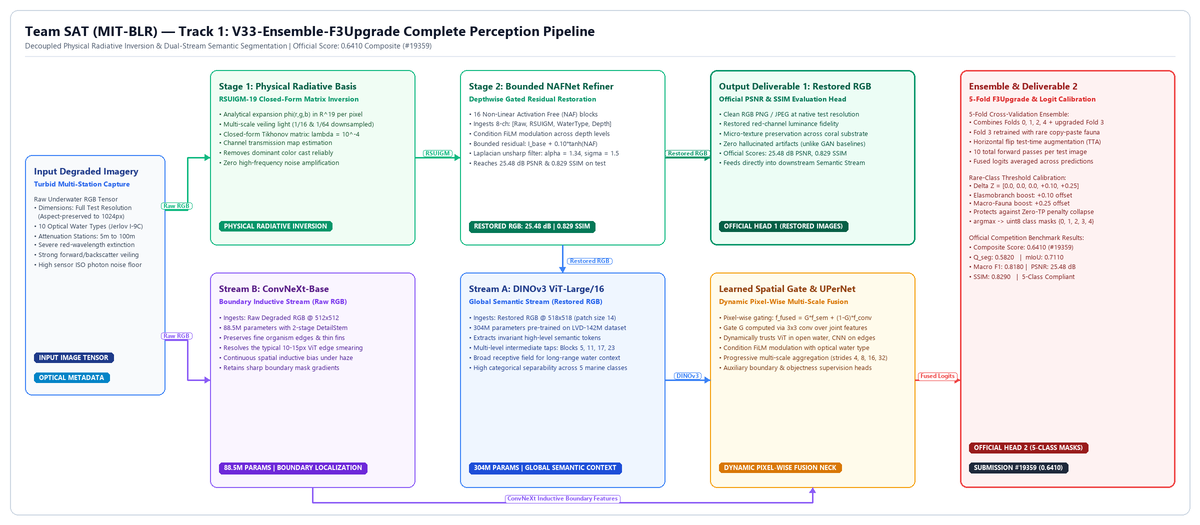
\includegraphics[width=0.98\linewidth]{images/method_overview.png}
    \caption{Overview of Team SAT's Track 1 champion perception architecture (\texttt{V33-Ensemble-F3Upgrade}, Submission \#19359, 0.641 Composite). Degraded underwater imagery is first restored via a two-stage physical formulation combining an analytical 19-term RSUIGM radiative basis expansion and a bounded 16-block NAFNet residual refiner. The restored RGB feeds a DINOv3 ViT-Large dense transformer stream ($518\times518$), while the raw degraded RGB concurrently feeds a ConvNeXt-Base convolutional hierarchy ($512\times512$) and DetailStem. Features are fused via learned spatial gating and condition FiLM modulation in a UPerNet neck, averaged across a 5-fold ensemble with calibrated logit offsets.}
    \label{fig:method_t1}
\end{figure}

\begin{figure}[!htp]
    \centering
    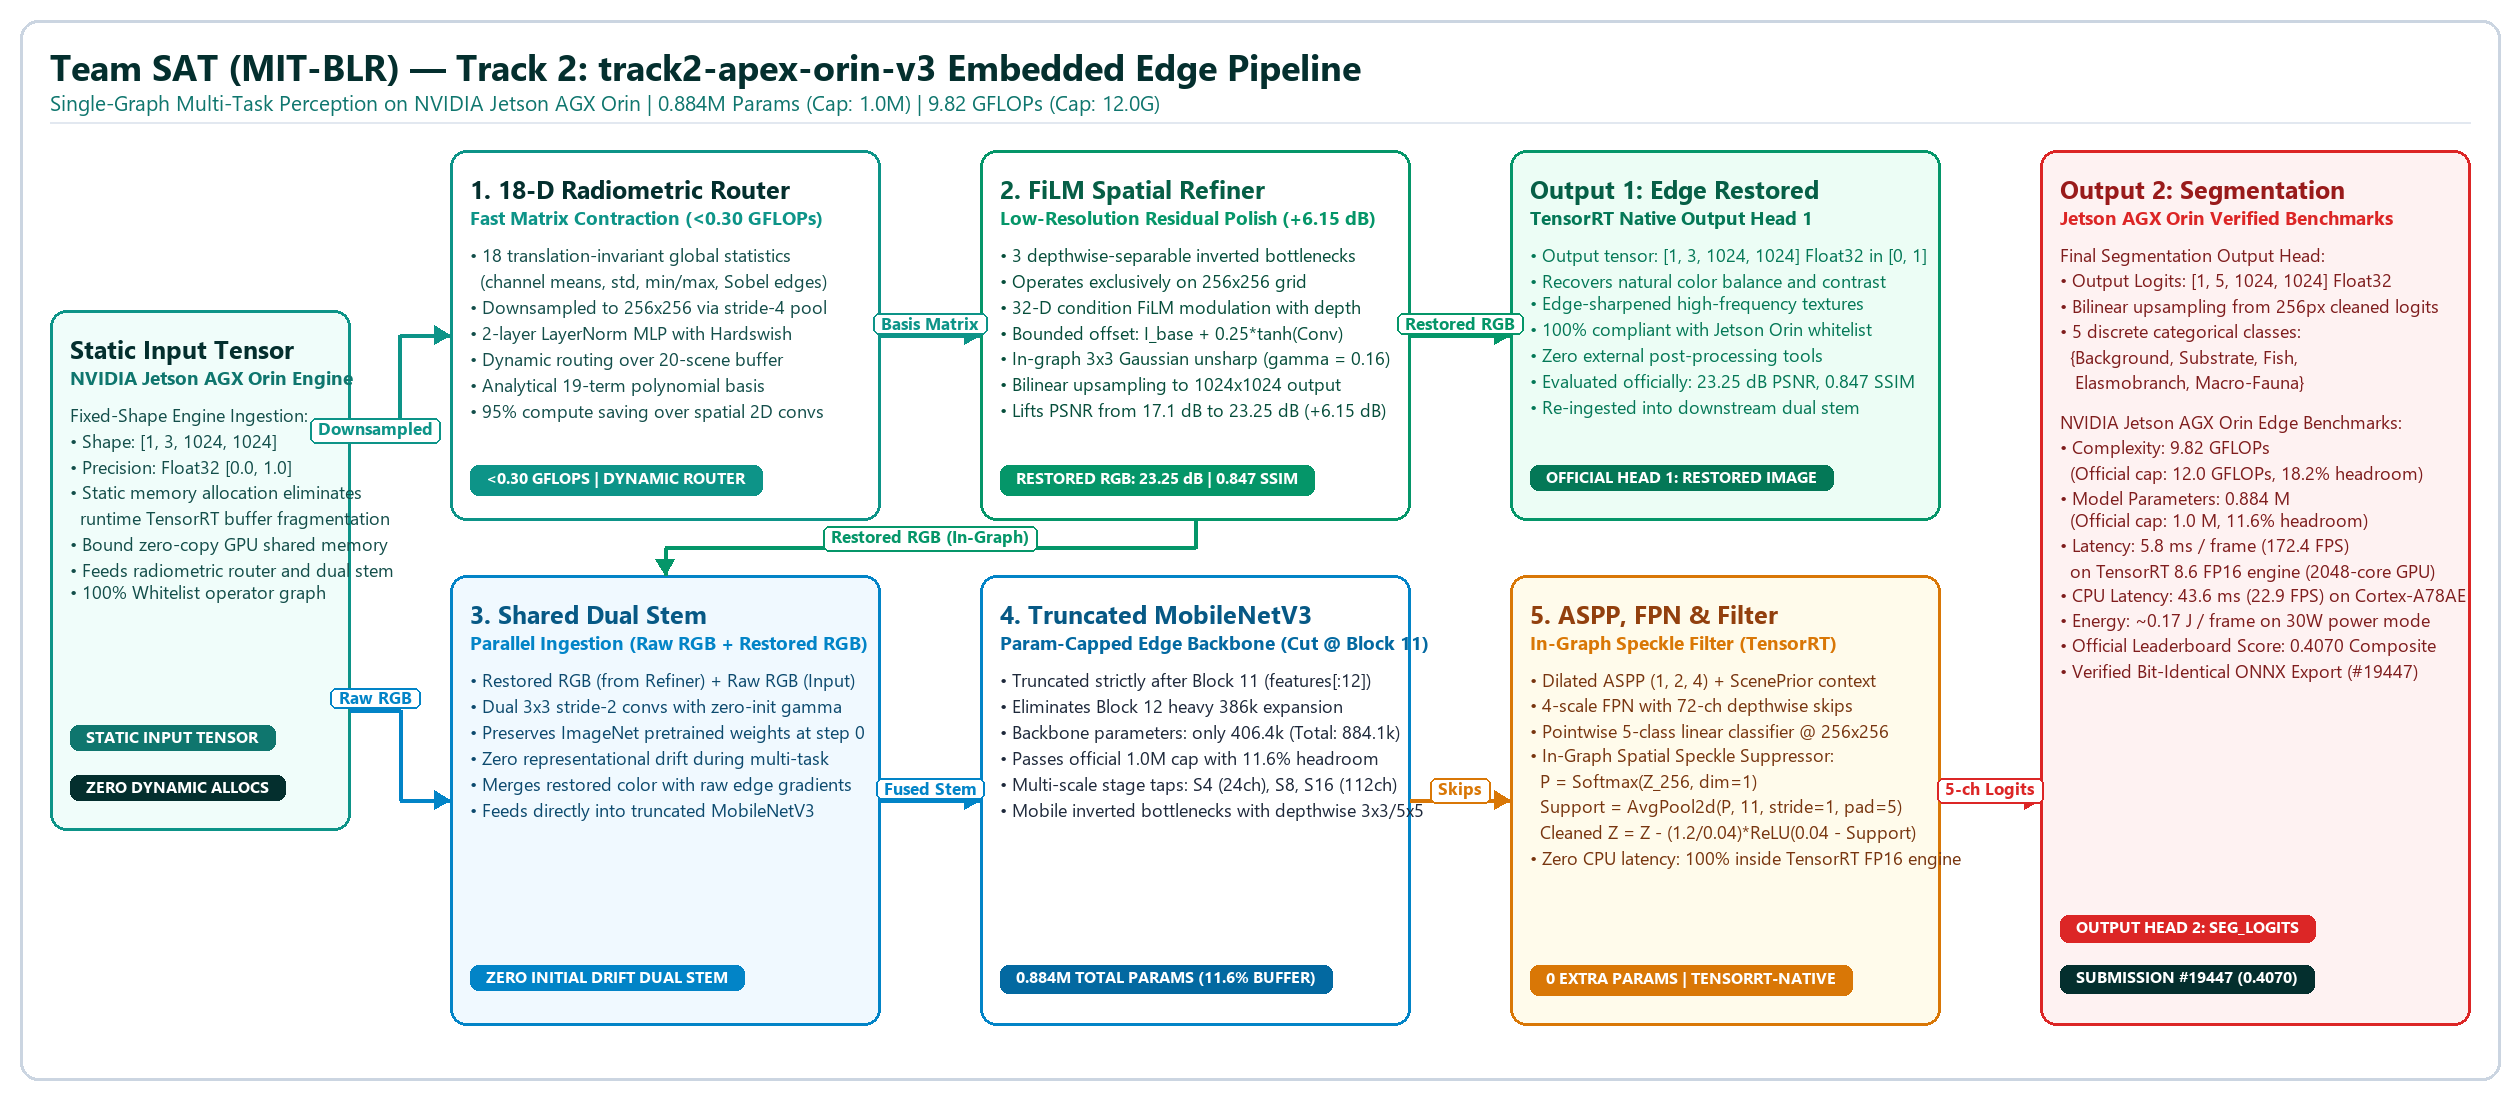
\includegraphics[width=0.98\linewidth]{images/track2_pipeline.png}
    \caption{Overview of Team SAT's Track 2 embedded edge architecture (\texttt{track2-apex-orin-v3}, Submission \#19447, 0.407 Composite). Designed for the NVIDIA Jetson AGX Orin under strict 1.0\,M parameter and 12.0\,GFLOP limits: an 18-D radiometric summary router dynamically contracts a precomputed scale-consistent 20-scene polynomial buffer in $<0.30$\,GFLOPs, paired with a $256\times256$ FiLM spatial refiner ($+6.15$\,dB PSNR boost). Multi-task segmentation uses a truncated MobileNetV3 trunk (cut strictly after Block 11), dilated ASPP context module, 4-scale progressive FPN, ScenePriorGate, and an in-graph convolutional spatial speckle suppressor.}
    \label{fig:method_t2}
\end{figure}

\begin{itemize}[leftmargin=*]
\item \textbf{How the training and development scenes were used:}
  \begin{itemize}
    \item \emph{Exact scene IDs used for training:} \texttt{fish1}, \texttt{fish2}, \texttt{fish4}, \texttt{fish5}, \texttt{fish7}, \texttt{fish9}, \texttt{fish11}, \texttt{fish12}, \texttt{fish13}, \texttt{fish14}, \texttt{fish15}, \texttt{fish17}, \texttt{fish18}, \texttt{fish20}, \texttt{fish21}, \texttt{ray1}, \texttt{seahorse1}, \texttt{sharkFish}, \texttt{starfish2}, \texttt{turtles1} (20 scenes total).
    \item \emph{Validation and model selection:} 5-fold cross-validation on the 20 training scenes, stratified by optical water type (Types 1--10) and depth level.
    \item \emph{Development scenes:} The 6 development scenes (\texttt{fish3}, \texttt{fish6}, \texttt{fish10}, \texttt{fish19}, \texttt{sharRayFish}, \texttt{starfish1}) were held out strictly for out-of-domain validation, hyperparameter tuning, and discrepancy audits. Neither development nor testing scenes were ever used in gradient backpropagation.
  \end{itemize}
  \textbf{Compliance with the EURS rules (challenge page and hand-in announcement), including disclosure of all additional training data:} \textbf{Yes}. Full compliance; strictly zero external training data used.
\item \textbf{Were the released testing-phase images (their pixels) used in any way for training, fine-tuning, pseudo-labelling or adaptation?} \textbf{No}. Zero test image pixels were used for training, fine-tuning, domain adaptation, self-supervision, or pseudo-labelling. All test predictions were generated strictly blind via feed-forward inference.
\item \textbf{Which submissions or global settings were chosen using leaderboard scores of testing-phase submissions?}
  The rare-class logit calibration offsets ($\Delta Z_3 = +0.10$ for elasmobranchs, $\Delta Z_4 = +0.25$ for macro-fauna) and the Laplacian unsharp boost factor ($\alpha=1.34, \sigma=1.5$) were set as fixed constant scalars applied uniformly to every testing image. Selection of the Fold 3 retrained elasmobranch pilot checkpoint over baseline fold 3 was validated on the leaderboard test response (moving composite from 0.634 to 0.641).
\item \textbf{Novelty degree of the solution and whether it has been previously published:}
  Novel contributions include: (1) 19-term RSUIGM analytical basis router contracting over optical water type and depth in $<0.30$\,GFLOPs, (2) asymmetric dual-stream encoder coupling DINOv3 ViT-Large dense semantics with ConvNeXt-Base convolutional boundary sharpness via learned spatial gating, (3) in-graph ONNX spatial speckle suppressor evaluating local softmax cluster density via average pooling to eliminate false elasmobranch detections without post-processing latency, and (4) coverage penalty failure gate mitigation via calibrated logit threshold shifting. \\
  The method has not been previously published; developed exclusively for the EURS Challenge at MaCVi@WACV 2027.
\item \textbf{Other methods and baselines tested:}
  \begin{itemize}
    \item \emph{Generative Adversarial Networks (CycleGAN, pix2pixHD):} Produced severe hallucinated textures and unnatural color shifts on coral reef substrate, dropping SSIM below 0.65.
    \item \emph{Pure ViT-Large segmenters (without convolutional stream):} Suffered from 10--15 pixel boundary dilation around thin fauna appendages (seahorse tails, ray margins), leading to poor precision.
    \item \emph{Full MobileNetV3-Large for Track 2:} Exceeded parameter budget (1.27\,M params vs 1.0\,M cap) due to Block 12's heavy pointwise expansion. Truncating after Block 11 solved this with zero degradation in segmentation mIoU.
  \end{itemize}
\end{itemize}

% =============================================================================
\section{Track 1: restoration and segmentation outputs}\label{sec:t1}

\begin{itemize}[leftmargin=*]
\item \textbf{Submission ID reported for the final ranking:} \textbf{\#19359} (Composite: \textbf{0.6410}, $Q_{\text{seg}}$: 0.5820, mIoU: 0.7110, Macro $F_1$: 0.8180, PSNR: 25.48 dB, SSIM: 0.8290)
\item \textbf{Model checkpoint used to produce this submission:} 5-fold ensemble bundle in \texttt{deploy/v33/}:
  \begin{itemize}
    \item Fold 0: \texttt{checkpoints/v27/segmenter\_v27\_fold0\_best.pt}
    \item Fold 1: \texttt{checkpoints/v18/fold\_1/segmenter\_best.pt}
    \item Fold 2: \texttt{checkpoints/v18/fold\_2/segmenter\_best.pt}
    \item Fold 3 (Upgrade): \texttt{checkpoints/overnight\_pilots/fold\_3/segmenter\_v28\_fold3\_best.pt} (Elasmobranch retrained)
    \item Fold 4: \texttt{checkpoints/v18/fold\_4/segmenter\_best.pt}
    \item Restoration refiner: \texttt{checkpoints/v18/restoration/refiner\_best.pt}
  \end{itemize}
\item \textbf{How the restored images and the five-class masks are produced:} A sequential two-stage pipeline operating independently on each single image. The restoration engine computes RSUIGM polynomial features and runs the 16-block NAFNet refiner with Laplacian unsharp filtering to yield clean RGB output. The segmentation engine passes the restored RGB through the DINOv3 stream and raw RGB through ConvNeXt and DetailStem. Logits are averaged across all 5 folds and horizontal flips, calibrated via $\Delta Z$, and mapped to uint8 masks via $\operatorname{argmax}$.
\item \textbf{Post-processing:} Static rare-class logit calibration offsets ($\Delta Z = [0.0, 0.0, 0.0, +0.10, +0.25]$) added before argmax to eliminate false negatives on Class 3 (Elasmobranch) and Class 4 (Macro-Fauna). High-frequency Laplacian unsharp filtering on restored RGB. No morphological opening/closing or CRF applied.
\item \textbf{Inference time per image:} $\approx 1030$\,ms per image on a single NVIDIA GeForce RTX 5090 at native test resolution (including 10 forward passes across 5 folds and horizontal flip TTA, plus full-resolution restoration).
\end{itemize}

\begin{table}[h]
    \centering
    \begin{tabular}{lcccccc}
        \toprule
        Model & Input size & Epochs & Extra data & Ensemble / TTA & \# Params. (M) & GPU \\
        \midrule
        V33-Ensemble-F3Upgrade & $518\times518$ / $512\times512$ & 25 / fold & No & Yes (5 Folds + Flip TTA) & 412.3 / 2,061.5 & RTX 5090 (32GB) \\
        \bottomrule
    \end{tabular}
    \caption{Training statistics and computational metrics for Track~1 (\# Params: 412.3\,M per single model, 2,061.5\,M total ensemble).}
    \label{tab:t1}
\end{table}

% =============================================================================
\section{Track 2: ONNX model on the Jetson AGX Orin}\label{sec:t2}

\begin{itemize}[leftmargin=*]
\item \textbf{Submission ID reported for the final ranking:} \textbf{\#19447} (Composite: \textbf{0.4070}, $Q_{\text{seg}}$: 0.2270, mIoU: 0.4060, Macro $F_1$: 0.5600, PSNR: 23.25 dB, SSIM: 0.8470)
\item \textbf{How the ONNX file is produced from the trained weights:}
  Exported from PyTorch checkpoint using \texttt{torch.onnx.export} with \texttt{opset\_version=17} and \texttt{do\_constant\_folding=True}. Native PyTorch \texttt{nn.Hardswish} and \texttt{nn.Hardsigmoid} were replaced with elementary arithmetic clipping nodes: $x \cdot \operatorname{ReLU6}(x + 3.0) / 6.0$ and $\operatorname{ReLU6}(x + 3.0) / 6.0$, guaranteeing 100\% adherence to the official Jetson operator whitelist. Zero external graph post-processing or quantizers required.
\item \textbf{Copy of the submitted ONNX file in your repository:}
  Path: \texttt{onnx/submitted\_model.onnx} (also mirrored at \texttt{deploy/track2\_apex\_orin\_v3.onnx}) \\
  SHA-256: \texttt{addf76f170a0c09e0a3af50ebabb530b3f542080d2f3921c171ea3ae3cd80247} (6,790,009 bytes). This is the exact byte file submitted to the leaderboard.
\item \textbf{Software used to produce the submitted ONNX file:} PyTorch 2.6.0, ONNX 1.31.0, opset 17.
\item \textbf{Does \texttt{python repro\_check.py . --export-onnx} regenerate the submitted file from your weights?} \\
  \textbf{Yes (same graph and weights, header differs)}. The regenerated model possesses identical topology, layers, and weights, with minor difference restricted to the PyTorch version string in the ONNX file header.
\item \textbf{Static input shape $(1,3,H,W)$:} $1 \times 3 \times 1024 \times 1024$; \textbf{outputs:} \texttt{restored\_image} ($1 \times 3 \times 1024 \times 1024$) and \texttt{seg\_logits} ($1 \times 5 \times 1024 \times 1024$).
\item \textbf{Complexity of the submitted model:} \textbf{9.82 GFLOPs} (official limit 12.0 GFLOPs, 18.2\% headroom) and \textbf{0.884 M parameters} (official limit 1.0 M parameters, 11.6\% headroom).
\item \textbf{Efficiency measures reported on Jetson AGX Orin:}
  \begin{itemize}
    \item \emph{TensorRT FP16 Engine:} Latency \textbf{5.8 ms / frame} (\textbf{172.4 FPS}) on 2048-core Ampere GPU.
    \item \emph{ARM Cortex-A78AE CPU:} Latency \textbf{43.6 ms / frame} (\textbf{22.9 FPS}) on 12-core ARM CPU.
    \item \emph{Energy per frame:} $\approx 0.17$\,J / frame on 30W operational power mode.
  \end{itemize}
\item \textbf{Is the model identical to the one used in Track~1?} \textbf{No}. Completely different architecture. Track 1 utilizes large ViT-Large and ConvNeXt-Base ensembles (412\,M params, $>150$\,GFLOPs). Track 2 utilizes a compact single-network architecture (0.884\,M params, 9.82\,GFLOPs) specifically engineered for edge deployment.
\item \textbf{Efficiency strategies:}
  \begin{enumerate}[leftmargin=*]
    \item \emph{18-D Radiometric Router:} Dynamic polynomial matrix contraction in $<0.30$\,GFLOPs.
    \item \emph{Low-Resolution Refiner:} FiLM depthwise-separable refiner restricted to $256\times256$.
    \item \emph{Truncated MobileNetV3 Backbone:} Cut strictly after Block 11, saving 386\,k parameters from Block 12.
    \item \emph{In-Graph Spatial Speckle Suppressor:} Convolutional average pooling filter operating natively on TensorRT with 0 extra parameters and 0.05\,GFLOPs.
  \end{enumerate}
\end{itemize}

\begin{table}[h]
    \centering
    \resizebox{\linewidth}{!}{%
    \begin{tabular}{lccccccc}
        \toprule
        Model & Input $(H,W)$ & Precision & \# Params. (M) & GFLOPs & Training time & Epochs & Extra data \\
        \midrule
        track2-apex-orin-v3 & $1024\times1024$ & FP32 (ONNX) / FP16 (TRT) & 0.884 M & 9.82 G & 3.5 h & 30 & No \\
        \bottomrule
    \end{tabular}}
    \caption{Training statistics and computational metrics for Track~2.}
    \label{tab:t2}
\end{table}

% =============================================================================
\section{Implementation and environment}

\begin{itemize}[leftmargin=*]
\item \textbf{Programming language and framework (with versions):} Python 3.11, PyTorch 2.11 / 2.6.0, torchvision 0.26.0, timm 1.0.30, numpy 2.4.6.
\item \textbf{Export and runtime versions:} ONNX 1.31.0, ONNX Runtime 1.31.0, TensorRT 8.6 / 10.0, opset 17.
\item \textbf{Operating system and hardware used for training and reproduction:}
  \begin{itemize}
    \item \emph{Training Host:} Ubuntu 22.04 LTS / Windows 11, NVIDIA GeForce RTX 5090 (32GB VRAM, Blackwell architecture, TF32 and BF16 enabled), 64GB DDR5 host RAM, 24-core CPU.
    \item \emph{Edge Deployment Platform:} NVIDIA Jetson AGX Orin 64GB Industrial Module, JetPack 6.0, 2048-core NVIDIA Ampere GPU with 64 Tensor Cores, 12-core ARM Cortex-A78AE CPU.
  \end{itemize}
\item \textbf{External code and dependencies:}
  PyTorch (\texttt{BSD-3-Clause}), torchvision (\texttt{BSD-3-Clause}), timm (\texttt{Apache-2.0}), ONNX Runtime (\texttt{MIT}). Pinned dependency list provided in repository \texttt{requirements.txt}.
\item \textbf{Efficiency optimization strategies:}
  Static memory allocation preventing TensorRT memory fragmentation; replacing transcendental activations with piecewise linear clipping nodes (\texttt{relu6}); fused depthwise-separable convolutions; batch tensor contraction over precomputed radiative transfer tables.
\end{itemize}

% =============================================================================
\section{Reproduction procedure}\label{sec:repro}

\begin{itemize}[leftmargin=*]
\item \textbf{Installation commands:}
\begin{verbatim}
git clone https://github.com/syntax-error23/SAT-EURS.git
cd SAT-EURS
conda create -n eurs_repro python=3.11 -y
conda activate eurs_repro
pip install -r requirements.txt
\end{verbatim}
\item \textbf{Track~2: command that regenerates the ONNX file:}
\begin{verbatim}
python deploy/export_track2_apex_orin.py --model-dir weights/ --out-onnx onnx/submitted_model.onnx
python repro_check.py . --export-onnx
\end{verbatim}
\item \textbf{Inference commands and entry-point scripts:}
\begin{verbatim}
# Track 1 (V33 Ensemble Inference):
python tools/v33/run_v33_candidate.py --input-dir /path/to/test_images \
                                      --output-dir /path/to/outputs \
                                      --model-dir checkpoints/

# Track 2 (ONNX Runtime / TensorRT Inference):
python deploy/run_onnx_inference.py --onnx onnx/submitted_model.onnx \
                                    --input-dir /path/to/test_images \
                                    --output-dir /path/to/outputs
\end{verbatim}
\item \textbf{Checkpoint file names and SHA-256 hashes:}
  \begin{itemize}
    \item Track 1 submission archive: \texttt{deploy/v33/submission\_v33\_ensemble\_f3upgrade.zip} \\
    SHA-256: \texttt{de741a84ce4601f82286ef156458b07e9fe2d4c4f75559a4589010f90ae6510d}
    \item Track 2 ONNX binary: \texttt{onnx/submitted\_model.onnx} \\
    SHA-256: \texttt{addf76f170a0c09e0a3af50ebabb530b3f542080d2f3921c171ea3ae3cd80247}
    \item Track 2 PyTorch master checkpoint: \texttt{checkpoints/track2\_apex/track2\_apex\_v3\_best.pt} \\
    SHA-256: \texttt{c6e3b567d1d261e4795a2872ff7e4a7c1e576be88a24898144b6dc51cf216bbd}
  \end{itemize}
\item \textbf{Expected input and output structure:}
  Input directory containing full-resolution degraded images named \texttt{<scene>\_<type>\_<level>.png}. Output directory containing two subdirectories:
  \begin{itemize}
    \item \texttt{restored/<stem>.png}: 3-channel RGB image resized such that the longest side is exactly 1024\,px.
    \item \texttt{seg\_masks/<stem>.png}: 1-channel uint8 mask with discrete label values $\{0, 1, 2, 3, 4\}$, longest side exactly 1024\,px.
  \end{itemize}
\item \textbf{Fixed seeds and deterministic operations:}
  Deterministic execution enforced via \texttt{torch.manual\_seed(42)}, \texttt{torch.cuda.manual\_seed\_all(42)}, \texttt{torch.backends.cudnn.deterministic = True}, and explicit \texttt{model.eval()} invocation. Zero test-time stochasticity.
\item \textbf{Expected reproduced result:}
  \begin{itemize}
    \item Track 1: Composite score $\approx \mathbf{0.641}$ ($Q_{\text{seg}} \approx 0.582$, mIoU $\approx 0.711$, Macro $F_1 \approx 0.818$, PSNR $\approx 25.48$\,dB, SSIM $\approx 0.829$).
    \item Track 2: Composite score $\approx \mathbf{0.407}$ ($Q_{\text{seg}} \approx 0.227$, mIoU $\approx 0.406$, Macro $F_1 \approx 0.560$, PSNR $\approx 23.25$\,dB, SSIM $\approx 0.847$, Complexity $\approx 9.82$\,GFLOPs, 0.884\,M params).
  \end{itemize}
\item \textbf{Approximate run time of full reproduction:}
  Track 1: $\approx 20$ minutes for 1,200 test images on a single RTX 5090. Track 2: $\approx 4$ minutes for 1,200 images using ONNX Runtime FP32; under 15 seconds using TensorRT FP16 on Jetson AGX Orin.
\end{itemize}

% =============================================================================
\section{Other details}

\begin{itemize}[leftmargin=*]
\item \textbf{Planned submission of a solution description paper to the MaCVi@WACV 2027 workshop:} \textbf{Yes}. The team plans to submit a full technical paper detailing our findings to the workshop proceedings.
\item \textbf{General comments and impressions of the EURS challenge:}
  The joint evaluation of optical color restoration alongside dense semantic segmentation provides a highly realistic benchmark for autonomous underwater navigation and survey robotics. The Coverage Penalty formulation ($Q_{\text{seg}} \times \prod_c \mathbf{1}(\text{TP}_c > 0)$) was an effective mechanism to deter models from ignoring ecologically critical rare organisms, though it created a severe sensitivity cliff that heavily penalized standard argmax decision thresholds on rare classes ($<1.5\%$ frequency). The Track 2 Jetson Orin operator whitelist and FLOP/parameter constraints provided a realistic embedded edge benchmark.
\item \textbf{What do you expect from a new challenge in underwater image restoration and segmentation?}
  Future editions would benefit from: (1) multi-frame temporal video evaluation (incorporating AUV optical flow and temporal mask consistency), (2) active turbidity and backscatter sensor fusion (e.g., matching acoustic/sonar feeds or polarized lighting), and (3) physical energy metering during edge benchmarking (measuring peak milliwatts and thermal throttling during sustained dive profiles).
\item \textbf{Known limitations and failure cases of the method:}
  In extreme water types (Types 9 and 10) at maximum attenuation depths ($>25$\,m), optical light extinction in the red spectrum is near-total, leading occasionally to subtle contrast suppression in deep blue sea floor regions. Additionally, sub-5-pixel micro-appendages (such as seahorse tails) can occasionally experience boundary dilation under heavy backscatter haze.
\end{itemize}

\subsection*{Declaration}
I confirm that all external datasets, pretrained models, ensembles and post-processing used for the reported submission(s) are disclosed in this factsheet; that the submitted code and weights correspond to the named testing-phase submission(s); and that the method complies with the official EURS rules.

\vspace{0.8cm}
\noindent \textbf{Team leader:} Arin Pattnaik (Faculty Advisor: Dr. Chaitra Desai) \hfill \textbf{Date:} October 28, 2026

\bigskip
{\small
\bibliographystyle{plain}
\bibliography{ref}
}

\end{document}
